% imports
\documentclass[titlepage,twoside]{article}
\usepackage[utf8]{inputenc}
\usepackage[a4paper, total={16cm, 23cm}, top=3.5cm]{geometry}
\usepackage[dvipsnames]{xcolor}
\usepackage{
    amsmath,
    amssymb,
    amsthm,
    fancyhdr,
    siunitx,
    bm,
    lipsum,
    standalone,
    tikz,
    booktabs,
    enumitem,
    array,
}
\usepackage[colorlinks=true, allcolors=linkcolor]{hyperref}
\usepackage[nameinlink]{cleveref}
\usepackage[
    backend=biber,
    bibstyle=ext-authoryear,
    citestyle=ext-authoryear-comp,
    sorting=nyt,
    uniquename=false,
    maxbibnames=99,
    giveninits=true,
    sortcites=false,
]{biblatex}

% bibliographic options
\DeclareFieldFormat[article]{volume}{\mkbibbold{#1}}
\DeclareFieldFormat[article]{number}{\mkbibparens{#1}}
\DeclareFieldFormat[article]{pages}{#1}
\renewcommand*{\volnumdelim}{}
\renewbibmacro{in:}{}
\addbibresource{references.bib}
\DeclareFieldFormat{titlecase:title}{\MakeSentenceCase*{#1}}

% ref options
\crefname{section}{\S}{\S\S}
\crefname{subsection}{\S}{\S\S}
\crefname{equation}{}{}
\crefname{figure}{Figure}{Figures}
\newcommand\crefrangeconjunction{--}
\def\equationautorefname~#1\null{(#1)\null}
\numberwithin{equation}{section}
\definecolor{linkcolor}{RGB}{51, 54, 142}

\makeatletter
\patchcmd{\math@cr@@@align}{\cr}{\global\let\df@label\@empty\cr}{}{}
\makeatother

% page style options
\setlength{\oddsidemargin}{0cm}
\setlength{\evensidemargin}{0cm}
\pagestyle{fancy}
\fancyhead[LE,RO]{\bfseries\thepage}
\renewcommand{\sectionmark}[1]{\markboth{\MakeUppercase{\thesection.\ #1}}{}}
\fancyhead[RE,LO]{\bfseries\nouppercase{\leftmark}}
\fancyfoot{}

\renewcommand{\headrulewidth}{0.5pt}
\setlength{\headheight}{15pt}
\setlength\parindent{0pt}
\setlength\parskip{6pt}

% math macros
\renewcommand{\d}[1]{\mathrm{d}#1}
\newcommand{\diff}[2]{\frac{\mathrm{d} #1}{\mathrm{d} #2}}
\newcommand{\ddiff}[2]{\frac{\mathrm{d}^2 #1}{\mathrm{d} {#2}^2}}
\newcommand{\pdiff}[2]{\frac{\partial #1}{\partial #2}}
\renewcommand\vec{\bm}
\newcommand{\uvec}[1]{\vec{\hat{#1}}}
\newcommand{\grad}{\vec{\nabla}}
\newcommand{\prandtl}{\ensuremath{\mathrm{Pr}}}
\newcommand{\rayleigh}{\ensuremath{\mathrm{Ra}}}
\newcommand{\nusselt}{\ensuremath{\mathrm{Nu}}}
\renewcommand{\bar}[1]{\mkern 1.5mu\overline{\mkern-1.5mu#1\mkern-1.5mu}\mkern 1.5mu}

% text macros
\newcommand{\rb}{Rayleigh-B\'{e}nard}

\begin{document}
\begin{titlepage}
\vfill~

\begin{center}
    {\Huge \textbf{%
        Novel parametrisation techniques in weather and climate modelling and
        their evaluation using simpler analogue models
    }} \\
    \vspace{0.75cm}
    {\Large\textbf{Thomas D. Schanzer}} \\
    \vspace{6pt}
    {\large Supervisor: Prof. Steven Sherwood} \\
    \vspace{0.75cm}
    {\large%
        School of Physics

        Climate Change Research Centre and
        ARC Centre of Excellence for Climate Extremes

        University of New South Wales, Sydney, Australia
    }
\end{center}
\vfill
\begin{center}
{\large\textbf{Abstract}}

\begin{minipage}{13cm}
    Text
\end{minipage}
\end{center}
\vfill
\end{titlepage}

\newpage
\tableofcontents

\newpage
\pagestyle{fancy}
\thispagestyle{fancy}

\section{Introduction and background}
\subsection{The necessity of parametrisation}
% Broad introduction of weather/climate prediction and fluid equations
The primary task of general circulation models (GCMs) for Earth's weather and
climate is to simulate the dynamics of the atmosphere and ocean, which are
governed by the Navier-Stokes equations. The algorithm chosen to solve these
partial differential equations is known as a model's \emph{dynamical core}
\parencite{mcfarlane2011}. Since analytical solutions to the equations do not
exist, the dynamical core necessarily approximates the continuous equations
with finite-dimensional, exactly solvable alternatives using one of several
possible discretisation schemes (e.g., the finite difference, finite element,
finite volume and spectral methods) \parencite{christensen2022}. In practice,
this usually involves representing the prognostic variables (i.e., those that
affect the evolution of the flow) with sets of discrete samples in space and
time, whose resolution is constrained by the available computing resources. The
unavoidable consequence of discretisation is the loss of information about
processes occurring on spatial and temporal scales smaller than the
corresponding sampling intervals. These processes are said to be
\emph{unresolved}.

% why we need parametrisation: nonlinearity
It is tempting to na\"{i}vely accept the loss of fine-scale information as a
necessary sacrifice and hope the dynamical core will still make accurate
predictions for the larger, resolved scales. Unfortunately, this too is
impossible due to the \emph{nonlinearity} of the governing equations. It is
instructive to consider the linear case as a counterexample.

Linear differential equations allow arbitrary superpositions of solutions,
meaning that any given solution may be partitioned into high- and low-frequency
components, both of which are also solutions. One thus has the freedom to solve
for the low-frequency components alone without compromise. This property may be
understood more formally using the Fourier transform, defined for a function
$f$ of space and time by
\[
    \tilde{f}(\omega, \vec{k})
        = \int \d{t}\,\d^3{x}\, e^{i(\vec{k} \cdot \vec{x} - \omega t)}
        f(t, \vec{x}),
\]
which reduces any linear differential equation to an algebraic equation
relating the frequency $\omega$ to the wave vector $\vec{k}$. Each wavenumber
component of the initial state propagates trivially according to its own
time dependence $e^{-i(\vec{k} \cdot \vec{x} - \omega(\vec{k}) t)}$,
\emph{independently of the other components}. The fine-scale dynamics may
be safely neglected because they have no influence on the coarse scales.

The consequence of the nonlinearity of the equations governing atmospheric and
oceanic flows is, therefore, a coupling of the resolved coarse scales to the
unresolved fine scales \parencite{mcfarlane2011}.
% justification via Reynolds averaging
This fact may be demonstrated more explicitly by applying so-called
\emph{Reynolds averaging} to the equations \parencite{christensen2022}.
Reynolds averaging decomposes each field $q$ into the sum of a coarse-grained
(in space or time) or statistical-ensemble-averaged field $\bar{q}$ and a
perturbation $q'$. Note that $\bar{q'} = 0$ by definition. The coarse-graining
operation is assumed to be linear, commute with differentiation and satisfy
$\bar{\bar{p} q} = \bar{p} \bar{q}$ for any two fields $p$ and $q$
\parencite{monin2007}. Following the example given by
\textcite{christensen2022}, consider the incompressible Navier-Stokes
equations, which have the general form
\begin{align*}
    \pdiff{u_i}{t} + u_j \pdiff{u_i}{x_j} &= \sum f_i, \\
    \pdiff{u_i}{x_i} &= 0
\end{align*}
where $u_i$ are the components of the velocity, $x_i$ are the
coordinates and $f_i$ are various forces per unit mass. Summation over repeated
indices is implied. Applying the decomposition and coarse-graining both sides
of the equations yields
\begin{alignat*}{2}
    && \pdiff{}{x_i} \left( \bar{u_i} + u_i' \right) &= 0 \\
    \Rightarrow & \qquad &
        \pdiff{\bar{u_i}}{x_i}
        + \underbrace{\pdiff{\bar{u_i'}}{x_i}}_{=0} &= 0 \\
    \Rightarrow & \qquad &
        \pdiff{\bar{u_i}}{x_i} = \pdiff{u_i'}{x_i} &= 0
\end{alignat*}
and
\begin{alignat*}{2}
    && \sum \bar{f_i} &=
        \bar{\pdiff{}{t} \left( \bar{u_i} + u_i' \right)}
        + \bar{\left( \bar{u_j} + u_j' \right)
        \pdiff{}{x_j} \left( \bar{u_i} + u_i' \right)} \\
    &&&=
        \pdiff{\bar{u_i}}{t}
        + \underbrace{\pdiff{\bar{u_i'}}{t}}_{=0}
        + \bar{u_j} \pdiff{\bar{u_i}}{x_j}
        + \bar{u_j} \underbrace{\pdiff{\bar{u_i'}}{x_j}}_{=0}
        + \underbrace{\bar{u_j'}}_{=0} \pdiff{\bar{u_i}}{x_j}
        + \bar{u_j' \pdiff{u_i'}{x_j}} \\
    &&&=
        \pdiff{\bar{u_i}}{t} + \bar{u_j} \pdiff{\bar{u_i}}{x_j}
        + \pdiff{\bar{u_i' u_j'}}{x_j}
        - \bar{u_i' \underbrace{\pdiff{u_j'}{x_j}}_{=0}} \\
    \Leftrightarrow & \qquad &
        \pdiff{\bar{u_i}}{t} + \bar{u_j} \pdiff{\bar{u_i}}{x_j}
        &= \sum \bar{f_i} - \pdiff{\bar{u_i' u_j'}}{x_j}.
\end{alignat*}
The physical meaning of this last equation is that the evolution of the
coarse-grained velocity field depends not only on itself and the coarse-grained
forces, but also on the perturbations via $\bar{u_i' u_j'}$, which does not
necessarily vanish. This dependence is a consequence of nonlinearity.

The theoretical discussion in this section establishes that physical processes
occurring at one place in the spectrum of temporal and spatial scales are
coupled to all the other processes in the spectrum \parencite{franzke2015}. In
particular, to ignore the effect of processes not explicitly resolved in
numerical models would introduce unacceptable systematic biases, or errors, in
the model forecasts. GCMs therefore require parametrisation schemes to estimate
the effects of unresolved processes as functions of the available large-scale
information (and the parameters of these functions must be chosen
appropriately---hence the name ``parametrisation'').


\subsection{Mathematical formulation of the parametrisation problem}%
\label{sec:math}
In order to make any progress on the parametrization problem, it is necessary
to formalise the notion of estimating the ``effects'' of unresolved processes.
I will describe the general approach, which is well-established \parencite[see,
e.g.,][]{hasselmann1976,palmer2001,demaeyer2018,brajard2021}, while
acknowledging possible alternative conventions where they exist.

The Earth system may be considered as a dynamical system whose exact evolution
is governed by equations of the form
\begin{equation} \label{eqn:truth}
    \diff{\vec{z}}{t} = \vec{F}(\vec{z},t),
\end{equation}
where the vector $\vec{z}$ contains all the variables needed to fully specify
the state of the system and $\vec{F}$ is a nonlinear differential operator. One
then employs a change of variables $\vec{z} \to (\vec{x},\vec{y})$, where
$\vec{x}$ contains the information or variables that are explicitly resolved by
the model being studied and $\vec{y}$ contains the unresolved, `sub-grid'
information or variables. Practically, $\vec{x}$ and $\vec{y}$ can be thought
of as projections of the full state $\vec{z}$ onto lower-dimensional
subspaces \parencite{brajard2021}. Alternatively (and more concretely),
$\vec{x}$ can be obtained by averaging the original variables over several
adjacent grid points, with $\vec{y}$ being the corresponding residuals
\parencite{zacharuk2018,alcala2021}.

In principle, the change of variables splits \cref{eqn:truth}
into two parts
\begin{align*}
    \diff{\vec{x}}{t} &= \vec{G}(\vec{x},\vec{y},t), \\
    \diff{\vec{y}}{t} &= \vec{H}(\vec{x},\vec{y},t)
\end{align*}
that (still exactly) describe the coupled evolution of the resolved and
unresolved variables via nonlinear differential operators $\vec{G}$ and
$\vec{H}$. The goal of parametrisation is now to derive a new system of
equations
\begin{equation*}
    \diff{\tilde{\vec{x}}}{t} = \tilde{\vec{G}}(\tilde{\vec{x}},t)
\end{equation*}
whose solution $\tilde{\vec{x}}(t)$ approximates the true $\vec{x}(t)$ as well
as possible without explicitly modelling $\vec{y}(t)$. The measure used to
compare $\tilde{\vec{x}}$ and $\vec{x}$ depends on the intended function of the
parametrised model; weather forecasting applications that prioritise short-term
predictive skill might call for minimisation of the root-mean-square error
(RMSE), while climate prediction would be more concerned with the closeness of
long-term average quantities.

There are several possible interpretations of $\tilde{\vec{G}}(\vec{x},t)$ and
its relationship to $\vec{G}(\vec{x},\vec{y},t)$. \textcite{hasselmann1976}
describes $\tilde{\vec{G}}(\vec{x},t)$ as an ensemble average of
$\vec{G}(\vec{x},\vec{y},t)$, taken over the distribution of all $\vec{y}$ that
are possible for a given $\vec{x}$, i.e.
\begin{equation*}
    \tilde{\vec{G}}(\vec{x},t)
        = \langle \vec{G}(\vec{x},\vec{y},t) \rangle_{\vec{y}}.
\end{equation*}
\textcite{demaeyer2018} instead assert that the ultimate goal of
parametrisation is to literally approximate $\vec{y}$ as a function
$\vec{\xi}(\vec{x})$, in which case
\begin{equation*}
    \tilde{\vec{G}}(\vec{x},t)
        = \vec{G}(\vec{x},\vec{\xi}(\vec{x}),t).
\end{equation*}
In practice, $\vec{G}(\vec{x},\vec{y},t)$ usually separates into a known
resolved part $\vec{D}(\vec{x},t)$ independent of $\vec{y}$ and an unresolved
coupling term $\vec{C}(\vec{x},\vec{y},t)$. It then suffices to approximate
only the unresolved part by a parametrisation $\vec{P}(\vec{x}, t)$ using one
of the above methods, so that the parametrised model reads
\begin{equation} \label{eqn:parametrised_model}
    \diff{\tilde{\vec{x}}}{t}
        = \vec{D}(\tilde{\vec{x}},t) + \vec{P}(\tilde{\vec{x}}, t).
\end{equation}


\subsection{Physical processes requiring parametrisation}
% spectrum of scales and implications of cross-interaction
% Examples of processes requiring parametrisation
Following the broad theoretical argument in the previous sections, I now turn to
concrete examples of processes that are often represented by parametrisations,
restricting the discussion to atmospheric processes for brevity. This section
will give a basic introduction to each process, its effect on the larger-scale
behaviour of the climate system and the role of its corresponding
parametrisation scheme. The purpose of these examples is to provide real-world
context and motivation for current parametrisation research in more idealised
settings, which will form one of the main topics of this review.

\emph{Cloud microphysics} parametrisations model the composition of clouds in
terms of the amount of water in the solid (e.g., hail), liquid (cloud droplets
and rain) and gaseous phases, and the rate of transitions between these phases.
Accurate representation of cloud formation and evolution is crucial for several
reasons. First, the interaction of clouds with solar and terrestrial radiation
has a major influence on the overall energy balance of the atmosphere
\parencite{mcfarlane2011}. Second, cloud water phase transitions lead to the
formation of precipitation, and are a source and sink of latent heat that
drives convection \parencite{mcfarlane2011}. Furthermore, the statistics of
cloud formation are linked to global temperatures in a feedback loop;
uncertainty in the sign and magnitude of this feedback effect is a major
contributor to uncertainty in the sensitivity of global temperatures to
increases in atmospheric CO$_2$ concentration \parencite{andrews2012,
christensen2022,stevens2013}. Microphysical processes occur on the spatial
scales of single water droplets and ice particles---among the smallest scales
in the atmosphere. All atmospheric models must parametrise the amount of cloud
water in each phase, the size distribution and concentration of liquid and ice
particles, and the resulting rate and type (rain, hail, snow, etc.) of
precipitation \parencite{christensen2022}.

\emph{Moist convection} encompasses vertical motions in the atmosphere that are
accompanied (and driven) by phase changes of water, and must be parametrised
when it occurs on sub-grid scales. Moist convection is generally triggered by
warming and moistening at low levels, which create convective instability, and
is manifested by narrow updrafts and downdrafts that can rarely be resolved
explicitly \parencite{mcfarlane2011}. Convection transports heat and moisture
vertically, removing the instability and generating storms where the condensed
water falls out as precipitation; more broadly, it is a key component of the
global atmospheric circulation in spite of its small spatial scale
\parencite{christensen2022}.

It should be noted that parametrisation also encompasses estimation techniques
for processes that are too complex to model exactly for reasons unrelated to
spatial and temporal resolution \parencite{mcfarlane2011}. A good example of
such a process is \emph{radiative transfer}. Air and its constituent gases, as
well as clouds, absorb, emit, reflect and/or scatter solar and terrestrial
radiation. This leads to differential heating and cooling that drives the
atmospheric circulation. While the theory of radiative transfer is understood
well enough to allow precise calculations in principle, the prohibitive
computational cost of such calculations necessitates a parametrisation based on
simplifying assumptions (the details of which are beyond the scope of this
review) \parencite{christensen2022}.


\subsection{Traditional solutions to the problem and their limitations}%
\label{sec:traditional}
With the examples of cloud microphysics, moist convection and radiative
transfer in mind, I now broadly review the traditional approaches used to
construct parametrisation schemes in practice. In particular, this section will
identify the key assumptions upon which many traditional schemes are founded,
and the circumstances under which the assumptions may be violated. This will
motivate research into novel approaches.

% conceptual model (examples)
A parametrisation scheme is traditionally constructed by formulating a
simplfied, easily solvable and deterministic conceptual model of the physical
process in question. The solution of this model is then used to estimate the
effect of the process on the coarse-scale state of the parent model, known as
the \emph{unresolved tendency} \parencite{mcfarlane2011}. For example, the earliest convective
parametrisation was developed by \textcite{manabe1965} and simply assumed that
the net effect of convection is to relax the vertical structure of the
atmosphere towards a neutrally stable state whenever it becomes convectively
unstable.
% motivate data-driven parametrisation here?
One obvious deficiency of simple conceptual models is that they cannot possibly
capture the full range of variability in the processes they simulate. One major
branch of modern parametrisation research therefore studies \emph{data-driven}
schemes that instead use observational or high-resolution simulated data to fit
empirical models for the unresolved processes, naturally capturing a wider
range of variability \parencite{christensen2022}. Data-driven parametrisation
will be discussed in much further detail in the next section.

% grid-box mean and scale separation
In general, a traditional parametrisation scheme aims to capture the net
unresolved tendency due to all occurrences of the unresolved process (e.g., all
convective updrafts and downdrafts) within each grid cell of the parent model.
A deterministic prediction of this type is valid when each grid cell contains
many independent realisations whose varying contributions may be expected to
yield a reliable average tendency. This requires a \emph{scale separation}
between the unresolved process and the resolution of the parent model. Scale
separation breaks down when model development and increases in available
computing resources allow simulations at resolutions approaching the previously
unresolved scales. In this case, knowledge of the coarse-scale state cannot be
expected to uniquely determine the unresolved tendency because the process is
only realised a few times in each grid cell. The resulting (seemingly) random
nature of the true unresolved tendency motivates stochastic treatments
\parencite{mcfarlane2011,christensen2022,berner2017}. These will be discussed
in the next section.

% closure, quasi-equilibrium -> memory
The conceptual models core to traditional parametrisations usually contain free
parameters that are determined from the coarse-scale model state using
additional assumptions called \emph{closures}. Closures often postulate a state
of quasi-equilibrium between the unresolved processes and their large-scale
environment, such as a balance between the accumulation of convective available
potential energy (CAPE) and its removal by convection, or between the
horizontal convergence of moisture at low levels and its convective transport
to higher levels \parencite{mcfarlane2011,christensen2022,palmer2019}. However,
there is no guarantee that such an equilibrium exists; in fact, it has been
demonstrated that the CAPE balance is violated by fluctuations on sub-diurnal
time scales \parencite{donner2003} and by midlatitude continental convection
\parencite{zhang2002}. Newer parametrisation schemes have allowed departures
from equilibrium by representing the unresolved processes in a prognostic
rather than diagnostic manner (i.e., allowing the processes to have their own
self-governing time dependence rather than calculating them from the
large-scale state at each time step independently of their values at the
previous step) \parencite{rio2019,berner2017}. This creates \emph{memory} or
\emph{latency} in the parametrised tendencies, meaning that the tendencies have
some nonzero response time when subjected to sudden changes in the large-scale
state. Memory will be discussed further in the next section.

% ISSUES
Parametrisation schemes commonly suffer from several other issues that I will
briefly address here.
% division of processes -> unification
Firstly, while the division of the general atmospheric dynamics into a set of
separately parametrised processes (microphysics, convection, etc.) is
physically motivated, it remains somewhat arbitrary because these processes,
strictly speaking, form a continuum without well-defined boundaries
\parencite{christensen2022,mcfarlane2011}. It is a goal of contemporary
research to unify the parametrisations as much as possible.
% universality
Secondly, given the importance of future climate projections, it is natural to
ask whether the parametrisation schemes that have been developed and tuned on
today's climate remain valid as the climate changes over decade- to
century-long simulations. This is a matter of particular concern for
data-driven parametrisations, since there is little reason to trust empirical
models once they are extrapolated beyond the range of the data originally used
to fit them \parencite{christensen2022}.
% conservation laws
Finally, unless very special care is taken, parametrisation schemes can cause
the parent model to violate known physical conservation laws (e.g., mass,
energy and momentum) \parencite{christensen2022}. Efforts to resolve this issue
are ongoing.


\newpage
\section{Novel approaches to the parametrisation problem}
% ongoing issues, processes will remain unresolved
Since the 1990s, the limitations identified in \cref{sec:traditional} have
prompted many to reconsider the principles upon which parametrisation schemes
are founded. The main advance has been the development of stochastic
parametrisations that incorporate random noise in the predicted tendencies.
More recently, others have approached the problem from an entirely new
direction, developing data-driven parametrisations that learn to predict the
tendencies empirically. This section will introduce the stochastic and
data-driven approaches in general terms while omitting the technical details of
individual implementations, the aim being to contextualise and motivate the
study of these approaches in more idealised frameworks in \cref{sec:simple}.
Other methods (such as superparametrisation) exist but are beyond the scope of
this review.


\subsection{Stochastic parametrisation and memory}
The potential value of stochasticity for climate modelling was first
established by \textcite{hasselmann1976}, whose seminal paper sought to explain
the characteristics of long-term climate variability. Knowing that climate
depends on interactions between all components of the Earth system
(atmosphere, ocean, cryosphere, biosphere, etc.), \citeauthor{hasselmann1976}
argued that the effect of the more rapidly-evolving atmosphere on the other,
more slowly-varying components is that of a stochastic forcing. Owing to
their long response time, the slowly-varying components effectively integrate
this stochastic forcing, allowing long-term climate variability to be
characterised as a type of random walk process akin to the Brownian motion
of a massive particle in a fluid.

Further motivation for stochastic parametrisation in particular stems from the
need to reliably estimate uncertainties in weather forecasts and climate
projections. Weather forecasting centres typically propagate initial condition
uncertatinties (due to imperfect observations) through to the final forecast in
a Monte Carlo fashion, by initialising an ensemble of model runs with perturbed
initial conditions and measuring the spread of the resulting forecasts. It has
been observed that deterministic models produce systematically under-dispersed
ensembles that fail to span the range of actual weather outcomes, indicating
that these models are failing to capture additional sources of variability
\parencite{palmer2005,berner2017,palmer2019}. Knowing that poor scale
separation and departures from quasi-equilibrium should preclude deterministic
relationships between unresolved tendencies and the large-scale state (see
\cref{sec:traditional}), it should seem highly likely that deterministic
parametrisation contributes to this deficiency.

% should this go at the beginning of the subsection so we get the point quicker?
The principle of stochastic parametrisation is, therefore, that unresolved
tendencies should be randomly sampled from an appropriate distribution at each
point in space and time, not simply set to the mean of the distribution
\parencite{franzke2015}. This choice has now been theoretically justified using
statistical mechanical arguments; most notably,
\textcite{wouters2012,wouters2013} showed that, assuming a weak coupling to the
resolved variables, the effect of unresolved dynamics should be parametrised by
a combination of deterministic and stochastic terms, as well as a
\emph{non-Markovian} memory term depending on the past states of the resolved
variables.

The simplest and earliest approach to stochastic parametrisation is the method
of \emph{stochastically perturbed parametrisation tendencies} (SPPT), which
takes an existing deterministic parametrisation and randomly scales its output
with a multiplicative noise field \parencite{palmer2019,christensen2020}.
Re-using the notation of \cref{sec:math}, an SPPT model for the resolved
variables $\vec{x}$ takes the form
\begin{equation*}
    \diff{\vec{x}}{t} = \vec{D}(\vec{x},t) + (1 + e) \vec{P}(\vec{x}, t),
\end{equation*}
where $\vec{P}$ is the existing deterministic parametrisation and $e$ is a
random field with mean zero. The choice of multiplicative (and thus inherently
state-dependent) rather than additive noise is intuitively motivated by the
expectation that variability in the effect of unresolved processes should be
greatest when those processes are most active \parencite{franzke2015}.
\textcite{christensen2020} performed a comparison of high-resolution
simulations to parametrised single-column model output which justified the use
of multiplicative perturbations. Additionally, it has been argued that the
random field $e$ should spatially and temporally correlated (in contrast to
uncorrelated ``white'' noise) in order to emulate the organisation of
unresolved processes on larger scales and their persistence in time
\parencite{christensen2022,franzke2015}. In particular, perturbations that
explictly depend on their own past values constitute a type of memory, albeit
distinct from the memory term advocated by \textcite{wouters2012,wouters2013},
which would instead couple the perturbations to the past values of the
large-scale variables.

Stochastic parametrisations have several known advantages over their
deterministic counterparts, and are now implemented in operational weather
forecast models. They have been found to remedy the aforementioned issues of
ensemble underdispersion and prediction unreliability
\parencite{palmer2005,berner2017}, and (as of 2009) even make the skill of
five-day forecasts comparable to that of deterministically parametrised two-day
forecasts \parencite{palmer2019}. Despite the zero-mean nature of the noise, it
has been shown that stochastic parametrisations can reduce systematic model
biases (``noise-induced drift''; \textcite{palmer2005}) and stabilise the
simulation of regime-based behaviour (such as the El Ni\~{n}o-Southern
Oscillation) in the climate system \parencite{berner2017}.

Reviewing the field, \textcite{palmer2019} identifies outstanding issues for
further research. The main concern is the lack of rigour in most stochastic
schemes; SPPT, for example, modifies existing deterministic schemes \emph{ad
hoc} rather than incorporating stochasticity \emph{ab initio} in the
development process. More objective approaches are yet to gain widespread
acceptance. This motivates both data-driven methods and further testing
using simpler dynamical systems where objectivity is more feasible.


\subsection{Data-driven parametrisation and machine learning}
The fitting of predictive statistical models to data is, of course, ubiquitous
in the sciences, but attempts to use such models as parametrisation schemes and
couple them into fully fledged GCMs are a relatively new phenomenon---certainly
more so than stochastic parametrisations. The prerequisite for all data-driven
parametrisations is obviously training data: mathematically, an approximate
solution of \cref{eqn:truth} of sufficient accuracy and resolution to be
considered ``truth'' for the application at hand. Training data are typically
derived from high-resolution simulations, such as regional weather model runs
or large eddy simulations (LES). The other ingredient is the imperfect
low-resolution model that will later be augmented by parametrisation.

To generate an appreciation of how these data might be used to construct a
parametrisation in practice, I roughly follow the argument and notation of
\textcite{brajard2021}. Define a map $\mathcal{M}$ that takes each state
$\vec{z}(t)$ in the training dataset to the state $\vec{z}(t + \delta t)$ at
the next time step. Similarly, denote by $\mathcal{M}^\mathrm{r}$ the
low-resolution model (the superscript r meaning ``reduced''), which maps a
low-resolution state $\vec{x}(t)$ to a prediction for $\vec{x}(t + \Delta t)$,
where $\Delta t$ is not necessarily equal to $\delta t$ (usually larger). The
spaces of high- and low-resolution states, having different dimensions, may be
linked by an operator $\langle \cdot \rangle$ that projects high-resolution
states onto the low-resolution state space. Practically, the projection
operation is simply a coarse-graining of $\vec{z}$ by averaging values at
adjacent grid points to match the resolution of $\vec{x}$. Now, for each state
$\vec{z}$ in the training dataset, one may compute the difference
\begin{equation*}
    \vec{\epsilon}(\vec{z}) =
        \frac{
            \langle \mathcal{M}(\vec{z}) \rangle - \langle \vec{z} \rangle
        }{\delta t}
        - \frac{
            \mathcal{M}^\mathrm{r}(\langle \vec{z} \rangle)
            - \langle \vec{z} \rangle
        }{\Delta t}
\end{equation*}
between the coarse-grained true tendency (on the left) and the tendency
predicted by the coarse model when it sees the same state (on the right). This
is the unresolved tendency. Knowledge of $\langle \vec{z} \rangle$ alone does
not uniquely determine $\vec{\epsilon}$ because $\langle \mathcal{M}(\vec{z})
\rangle$ depends on the original $\vec{z}$. However, if one can fit a
statistical model $\vec{P}$ to the dataset of ($\langle \vec{z} \rangle$,
$\vec{\epsilon}$), then $-\vec{P}(\vec{x}(t)) \Delta t$ will be able to serve
as an estimate of the error incurred by the coarse model in predicting
$\vec{x}(t + \Delta t)$ given $\vec{x}(t)$. This motivates the construction of
a parametrised model $\mathcal{M}^\mathrm{p}$, defined by
\begin{equation*}
    \mathcal{M}^\mathrm{p}(\vec{x}) =
        \mathcal{M}^\mathrm{r}(\vec{x}) + \vec{P}(\vec{x}) \Delta t
\end{equation*}
that simply subtracts the estimated error at each time step of the coarse
model. In theory, the solution $\vec{x}(t)$ obtained by iteration of
$\mathcal{M}^\mathrm{p}$ will be more accurate than that obtained by
iteration of the unparametrised $\mathcal{M}^\mathrm{r}$.

The current method of choice for constructing $\vec{P}$ in weather and climate
modelling contexts is machine learning (ML). I will briefly introduce the key
concepts, strengths and weaknesses of ML, following \textcite{beucler2022}. ML
encompasses a broad class of algorithms that programmatically and autonomously
develop and apply rules for performing tasks, such as image classification,
removing the need for a human to explicitly program the rules. They do this
using supplied \emph{training data} that exemplify the task to be performed.
When it comes to data-driven parametrisation, the task is function
approximation or regression, and the relevant algorithms usually require a
training dataset of example inputs (i.e., coarse-scale variables)
\emph{labelled} with the desired outputs (i.e., unresolved tendencies). One
commonly-used class of algorithms called \emph{neural networks} consist of
layers of inter-communicating calculation nodes called neurons and learn to
approximate functions by optimising sets of weights associated with the
neurons. Another type of algorithm is the \emph{random forest}, which
approximates functions by passing the inputs through a series of nested
\texttt{if/else} decision trees.

The distinguishing advantage offered by ML data-driven parametrisations is
their ability to systematically capture complex relationships without relying
on artificially simplified physical models derived by humans
\parencite{irrgang2021,beucler2022}. In addition to constructing new
parametrisations from scratch, ML has been used to emulate the action of
existing parametrisation schemes in weather and climate models
\parencite[e.g.,][]{gentine2018}. These ML emulators have the potential to
reduce the computational burden that parametrisation usually imposes, leaving
more resources for other tasks such as calling the parametrisation scheme more
frequently or increasing the model resolution \parencite{beucler2022}.
Furthermore, the ability to emulate multiple existing schemes at once is a step
towards unifying the parametrisation of unresolved processes (a long-standing
issue; see \cref{sec:traditional}).

ML parametrisations are not without their issues; they are known to be prone to
overfitting and often cause their host models to become numerically unstable.
They are also, by their very nature, far more difficult to interpret than
traditional schemes. It is therefore very difficult to determine \emph{a
priori} whether or not they will continue to be valid in climate conditions
outside the bounds of their training datasets
\parencite{irrgang2021,beucler2022}. ``Interpretable'' or ``explainable'' ML is
an active area of research that aims to address these issues. Another active
research topic is ``physics-guided ML'', the aim of which is to augment ML with
known physical constraints and conservation laws that would otherwise be
violated \parencite[e.g.,][]{yuval2021}.


\newpage
\section{Simple dynamical systems as testbeds for novel approaches}%
\label{sec:simple}


\newpage
\section{Dynamical system case study: \rb{} convection}
\subsection{Problem statement}
\rb{} convection is the motion of a fluid confined between two
horizontal isothermal plates, the temperature of the bottom plate being
higher than that of the top plate. The governing equations for the flow
follow from the Navier-Stokes equations of mass, energy and momentum
conservation. The reader is referred to \textcite{chandrasekhar1961} for
a detailed derivation; I summarise the assumptions and approximations
involved below.

The density, $\rho$, of the fluid is related to its temperature $T$ by
the linear equation of state
\[
    \rho = \rho_0 [1 - \alpha(T - T_0)],
\]
where $\alpha$ is the (constant) volume coefficient of thermal expansion and
$\rho_0$ and $T_0$ are the base-state density and temperature such that $\rho =
\rho_0$ when $T = T_0$. The key assumption is that density variations are small
($\alpha (T - T_0) \ll 1$), which allows the governing equations to be
simplified under the \emph{Boussinesq approximation}. The Boussinesq
approximation involves first writing the pressure, $p$, of the fluid as
\[
    p = p_0 - \rho_0 gz + p',
\]
where $p_0$ is an arbitrary constant, $g$ is the acceleration due to gravity
and $z$ is the vertical coordinate. $p'$ is the (time-varying) deviation from
a hydrostatically balanced background profile $p_0 - \rho_0 gz$
in which the upward pressure gradient force per unit volume $\rho_0 g$ cancels
the downward weight force per unit volume $-\rho_0 g$. Since
$\alpha (T - T_0) \ll 1$, density variations are neglected everywhere except
in their contribution to the weight force, leading to a net buoyant
(background pressure gradient plus weight) force per unit mass
\[
    \frac{\rho_0 - \rho}{\rho_0} g = \alpha (T - T_0) g.
\]

With these assumptions in mind, I adopt the governing equations as they
are derived by \textcite{chandrasekhar1961}:
\begin{alignat}{2}
    \label{eqn:dim_momentum}
    \pdiff{\vec{u}}{t} + \vec{u} \cdot \grad \vec{u}
        &= -\frac{1}{\rho_0} \grad p' + \alpha (T - T_0) g \uvec{z}
        + \nu \nabla^2 \vec{u}
    &\quad& \text{(momentum conservation),} \\
    \label{eqn:dim_energy}
    \pdiff{T}{t} + \vec{u} \cdot \grad T
        &= \kappa \nabla^2 T
    && \text{(energy conservation), and} \\
    \label{eqn:dim_incompressible}
    \grad \cdot \vec{u} &= 0
    && \text{(incompressibility).}
\end{alignat}
$\vec{u}$ is the fluid velocity, $t$ is time, $\uvec{z}$ is the upward
unit vector, $\nu$ is the (constant) kinematic viscosity and $\kappa$ is
the thermal diffusivity (also constant). Notice that the aforementioned
buoyancy term $\alpha (T - T_0) g$ appears on the right-hand side of
\cref{eqn:dim_momentum}.

The parametrisation test-bed developed in this work solves the governing
equations in a two-dimensional domain $(x,z) \in [0, d] \times [0, L]$, subject
to no-slip, isothermal boundary conditions on the top and bottom plates,
\begin{alignat}{3}
    \label{eqn:dim_bc_bot}
    \vec{u} &= \vec{0}, &\quad T &= T_0 + \frac{\delta T}{2}
    &\qquad& \text{at } z = 0 \text{ and} \\
    \label{eqn:dim_bc_top}
    \vec{u} &= \vec{0}, &\quad T &= T_0 - \frac{\delta T}{2}
    &\qquad& \text{at } z = d,
\end{alignat}
and periodic boundary conditions in the horizontal,
\begin{alignat}{2}
    \label{eqn:dim_bc_sides}
    \vec{u}(x=0) &= \vec{u}(x=L) &\quad \text{and} \quad T(x=0) &= T(x=L).
\end{alignat}
$\delta T$ is the constant temperature difference between the plates.

\subsection{Nondimensionalisation and scale analysis}
It is helpful to nondimensionalise the governing equations
\crefrange{eqn:dim_momentum}{eqn:dim_bc_sides}; this is not only useful for
numerical work but also gives insight into the different flow regimes that are
possible. A range of nondimensionalisations are used in fluid dynamics
literature; I adopt a common one \parencite[see,
e.g.,][]{grotzbach1983,ouertatani2008,stevens2010} which is suitable for the
turbulent convective regime.

For low-viscosity, turbulent flow, a suitable time scale is the
\emph{free-fall time} $t_0$, which is the time for a fluid element with
constant temperature $T = T_0 - \delta T$ to fall from the top plate to
the bottom plate under the influence of buoyancy ($-g \alpha \delta T$)
alone. It is simple to show that
\[
    t_0 \sim \left( \frac{d}{g \alpha \delta T} \right)^{1/2},
\]
ignoring a factor of $\sqrt{2}$. The obvious length and temperature
scales are the plate separation $d$ and temperature difference $\delta T$,
respectively.

Making the substitutions $p'/\rho_0 \to \pi$ and $T - T_0 \to \theta$
in \crefrange{eqn:dim_momentum}{eqn:dim_bc_sides} and expressing all
variables in units of $t_0$, $d$ and $\delta T$ leads to the dimensionless
equations
\begin{align}
    \label{eqn:momentum}
    \pdiff{\vec{u}}{t} + \vec{u} \cdot \grad \vec{u}
        &= -\grad \pi + \left( \frac{\prandtl}{\rayleigh}\right)^{1/2}
        \nabla^2 \vec{u} + \theta \uvec{z}, \\
    \label{eqn:energy}
    \pdiff{\theta}{t} + \vec{u} \cdot \grad \theta
        &= (\rayleigh\,\prandtl)^{-1/2} \, \nabla^2 \theta, \quad \text{and} \\
    \label{eqn:incompressible}
    \grad \cdot \vec{u} &= 0,
\end{align}
with boundary conditions
\begin{gather}
\begin{alignat}{3}
    \label{eqn:bc_bot}
    \vec{u} &= \vec{0}, &\quad \theta &= +\frac{1}{2}
    &\qquad& \text{at } z = 0, \\
    \label{eqn:bc_top}
    \vec{u} &= \vec{0}, &\quad \theta &= -\frac{1}{2}
    &\qquad& \text{at } z = 1,
\end{alignat} \\
\begin{alignat}{2}
    \label{eqn:bc_sides}
    \vec{u}(x=0) &= \vec{u}(x=\Gamma)
    &\quad \text{and} \quad \theta(x=0) &= \theta(x=\Gamma).
\end{alignat}
\end{gather}
There are three dimensionless parameters: the aspect ratio of the domain
\[
    \Gamma \equiv \frac{L}{d},
\]
the \emph{Prandtl number}
\[
    \prandtl \equiv \frac{\nu}{\kappa}
\]
which measures the relative importance of viscosity (momentum diffusivity)
and thermal diffusivity, and the \emph{Rayleigh number}
\[
    \rayleigh \equiv \frac{g \alpha d^3 \delta T}{\kappa \nu}.
\]
The Rayleigh number can be interpreted as the ratio of the time scale for
thermal transport by convection to the time scale for thermal transport by
conduction. It determines the importance of diffusion for the evolution of
$\vec{u}$ and $\theta$; inspection of \cref{eqn:momentum,eqn:energy} indicates
that low $\rayleigh$ implies strong diffusion and high $\rayleigh$ weak
diffusion. Detailed theoretical analysis of the governing equations (see, e.g.,
\textcite{chandrasekhar1961} and the seminal work by \textcite{rayleigh1916})
reveals that there exists a critical Rayleigh number (dependent on boundary
conditions but of order $\SI{e3}{}$), below which the equations have a stable
equilibrium with the fluid at rest and a linear conductive temperature profile.
Above the critical value, the equilibrium is unstable and small perturbations
lead to the formation of a regular series of steady, rotating convection cells.
If the Rayleigh number is increased much further (\textcite{le_quere1991} cites
$\rayleigh \approx \SI{2e8}{}$), the solution becomes unsteady and increasingly
turbulent. This work is concerned with the turbulent regime, since Rayleigh
numbers for atmospheric deep moist convection can be as large as $\SI{e22}{}$
\parencite{chilla2012}.

\subsection{Thermal properties}
The rate of heat transport across the fluid layer has physical significance for
natural realisations of thermally driven convection. It is widely analysed in
terms of the dimensionless \emph{Nusselt number}, whose accurate determination
is a common theme in the \rb{} convection literature; I therefore introduce
this quantity before proceeding. The Nusselt number measures the rate of
(vertical) heat transport across a horizontal plane at height $z$, normalised
by the purely conductive rate that would exist if the fluid were at rest
\parencite{verzicco1999}. Following \textcite{chilla2012}, I use the definition
(before nondimensionalisation)
\begin{equation}
    \label{eqn:dim_nusselt}
    \nusselt(z,t) \equiv \frac{
        \langle wT \rangle_{A,t}
        - \kappa \partial \langle T \rangle_{A,t} / \partial z
    }{
        \kappa \delta T / d
    }
\end{equation}
where $\langle \cdot \rangle_{A,t}$ denotes averaging over time and the
horizontal plane at height $z$, and $w = \vec{u} \cdot \uvec{z}$ is the
vertical velocity. The rate of heat transport in the numerator has two terms:
advection $\langle wT \rangle_{A,t}$ and conduction $-\kappa \partial \langle T
\rangle_{A,t} / \partial z$. The denominator $\kappa \delta T / d$ is the rate
of heat transport for a linear conductive temperature profile with the fluid at
rest. \textcite{scheel2013} give the corresponding nondimensionalised form,
\begin{equation}
    \label{eqn:nusselt}
    \nusselt(z,t) \equiv (\rayleigh\,\prandtl)^{1/2}
        \langle w \theta \rangle_{A,t}
        - \pdiff{\langle \theta \rangle_{A,t}}{z}.
\end{equation}

Another important quantity is the thickness $\delta_T$ of the \emph{thermal
boundary layer} at each plate where large temperature gradients exist.
\textcite{chilla2012} define $\delta_T$ as follows: if, on average, the fluid
temperature changes with height from $+\delta T/2$ at the lower plate to $0$
(the mean value in the well-mixed interior) over a distance $\delta_T$, then
\[
    \left. \pdiff{\langle T \rangle_{A,t}}{z} \right|_{z=0}
        \approx -\frac{\delta T}{2 \delta_T}.
\]
But if one considers the definition of the Nusselt number
\cref{eqn:dim_nusselt} at $z=0$, the advection term $\langle wT \rangle_{A,t}$
vanishes due to the $\vec{u} = \vec{0}$ boundary condition and
\[
    \nusselt(z=0) = -\frac{d}{\delta T}
        \left. \pdiff{\langle T \rangle_{A,t}}{z} \right|_{z=0}.
\]
Thus,
\begin{equation}
    \label{eqn:thermal_bl}
    \delta_T = \frac{d}{2\,\nusselt(z=0)}.
\end{equation}


\subsection{Resolution dependence of numerical solutions}
% s.sherwood: Might be important to further explain here that you will regard
% this as the ("warts and all") dynamical system you want to emulate at a
% coarser representation.  This avoids the issue of whether this hig-res is a
% perfect solution of the fluid equations or not (it doesn't have to be,
% although for robustness we want it to be relatively insensitive to small
% changes in dx).
In constructing a parametrisation test-bed, I will firstly seek
reasonably accurate, high-resolution ``truth'' solutions of
\crefrange{eqn:momentum}{eqn:bc_sides}. I will then deliberately reduce
the resolution, aiming to produce solutions that are sufficiently
``different'' that they might reasonably be ``improved'' by a parametrisation
scheme. In this section, I review relevant literature with the aim of
establishing how, exactly, under-resolved simulations of \rb{} convection
might ``differ'' from well-resolved ones, and thus what one would hope to
``improve''. Specifically, I will address the following questions:
\begin{itemize}
    \item What resolution is necessary for a converged solution?
    \item Which quantities are most sensitive to insufficient resolution?
\end{itemize}

\subsubsection{Theoretical resolution requirements for accurate simulations}%
\label{sec:res_requirements}

% resolution in general, Grotzbach condition.
\textcite{grotzbach1983} is recognised as the first to formulate resolution
requirements for accurate simulations of \rb{} convection
\parencite{chilla2012,scheel2013}. He identified separate constraints on the
mean (i.e., averaged in each spatial direction) grid spacing and the vertical
spacing near the plates; I first discuss the former.
\citeauthor{grotzbach1983} reasoned that a numerical model that neglects
subgrid-scale effects must have a geometric mean grid spacing $h = (\Delta x
\Delta y \Delta z)^{1/3}$ such that
\begin{equation}
    \label{eqn:grotzbach}
    h \leq \pi \eta = \pi \left(
        \frac{\nu^3}{\langle \epsilon \rangle}
    \right)^{1/4}
\end{equation}
where $\eta \equiv (\nu^3/\epsilon)^{1/4}$ is the \emph{Kolmogorov length}, the
universal smallest relevant length scale for general turbulent flow, and
$\langle \epsilon \rangle$ is the spatial and temporal average of the kinetic
energy dissipation rate defined by
\begin{equation}
    \label{eqn:kinetic_dissipation}
    \epsilon(\vec{x}, t) \equiv \frac{\nu}{2} \sum_{ij} \left(
        \pdiff{u_i}{x_j} + \pdiff{u_j}{x_i}
    \right)^2
\end{equation}
\parencite{chilla2012}. The condition \cref{eqn:grotzbach} can be
understood using the Nyquist-Shannon theorem, which states that a
sampling frequency $f \geq k/\pi$ is needed to unambiguously reconstruct
a signal with maximum wavenumber $k$; substituting $f = 1/h$, $k =
1/\eta$ leads to the claimed relation.

% resolution near plates, number of points.
\citeauthor{grotzbach1983} recognised that the above reasoning was only valid
for the mean grid spacing; large gradients in temperature and velocity near the
top and bottom plates require finer resolution in those regions. The notion of
nearness can be formalised using the thermal boundary layer thickness
\cref{eqn:thermal_bl}, and one asks how many grid points are necessary in this
layer. \citeauthor{grotzbach1983} did not give a theoretical argument to derive
this number but claimed that 3 points are sufficient for turbulent flows.
\textcite{shishkina2010} presented a theoretical argument based on the
(experimentally and numerically justified) assumption of laminar
\emph{Prandtl-Blasius} flow conditions in the boundary layer and were able to
calculate the minimum number of grid points (e.g., 9 for $\rayleigh =
\SI{2e9}{}$ and $\prandtl = 0.7$). The results agreed with criteria derived in
previous numerical experiments. Importantly, the results of
\citeauthor{shishkina2010} allow \emph{a priori} determination of vertical
resolution requirements, potentially bypassing the time-consuming and expensive
process of iteratively running simulations, checking their convergence and
updating the resolution.

\subsubsection{
    Resolution-dependence tests and consequences of under-resolution}%
\label{sec:res_tests}

Performing numerical experiments for a 3D fluid layer,
\citeauthor{grotzbach1983} found that RMS velocity and Nusselt number were
the most sensitive quantities to insufficient mean grid spacing, but even
they increased ``only slightly'' above the values obtained from well-resolved
simulations. He concluded that condition \cref{eqn:grotzbach} was overly
restrictive and recommended (for $\prandtl > 0.59$) the simplified,
approximate version
\[ % is this necessary?
    h \lesssim 5.23 \, \prandtl^{-1/4} \rayleigh^{-0.3205}.
\]
Later work also supports the finding that the Nusselt number is
sensitive to under-resolution. Even studying only steady-state convective
solutions at moderate Rayleigh number, \textcite{le_quere1991} found that the
maximum and minimum Nusselt numbers were most sensitive to changes in
resolution and had the largest uncertainty among existing benchmark solutions.
% ouertatani: common to use Nu as convergence test
Other studies have used the convergence of the Nusselt number as an indicator
that the spatial resolution is sufficient to produce an accurate solution
\parencite{ouertatani2008}.

\textcite{stevens2010} performed 3D simulations in a finite cylindrical cavity
with the aim of reconciling the apparent disagreement between the Nusselt
numbers in previous numerical studies and experimental observations. They found
that agreement with experiment could be achieved, but only by using a much
higher resolution than the previous studies. They offered the physical
explanation that horizontally under-resolved simulations produce insufficient
thermal diffusion, leading to systematic overestimation of the buoyancy of
convective plumes near the side-walls of the cylinder; this results in Nusselt
numbers that exceed experimentally observed values. This led them to conclude
that the two criteria of \textcite{grotzbach1983}---for mean grid spacing
and for the vertical spacing near the upper and lower plates---are not
independent; the definition $h = (\Delta x \Delta y \Delta z)^{1/3}$ in
\cref{eqn:grotzbach} allows the horizontal spacing to remain relatively
coarse near the plates, provided the vertical spacing is small. Since
fine horizontal resolution is also necessary to accurately capture
the dynamics of the thin plumes, they proposed that \cref{eqn:grotzbach} be
applied with $h = \max(\Delta x, \Delta y, \Delta z)$ instead.

% kooij: Nu may not be best indicator
Some more recent work, however, casts doubt on the notion that the Nusselt
number is sensitive to under-resolution and that its convergence is a good
indicator that the flow is well-resolved. In assessing the performance of
several published computational fluid dynamics codes on the \rb{} problem in a
cylindrical cavity, \textcite{kooij2018} identified one higher-order code that
reproduced the theoretically predicted scaling of $\nusselt$ as a function of
$\rayleigh$ even when the flow was deliberately under-resolved. On the other
hand, the presence of numerical artefacts in the instantaneous temperature
field near the bottom plate was a clear indicator of insufficient resolution.
\cref{fig:kooij2018_artefacts}, a reproduction of part of their Figure 5, shows
these artefacts.

% scheel: dissipation rates sensitive
\textcite{scheel2013} performed similar high-resolution simulations for
a cylindrical cavity and also found that the Nusselt number, among other
global transport properties, were ``fairly insensitive to insufficient
resolution, as long as the mean Kolmogorov length [was] resolved'' (i.e.,
\cref{eqn:grotzbach} was satisfied). However, they found that the horizontally
averaged or local kinetic energy dissipation rate
\cref{eqn:kinetic_dissipation} and the corresponding thermal dissipation rate
\begin{equation}
    \label{eqn:thermal_dissipation}
    \epsilon_T(\vec{x}, t) \equiv \kappa \sum_i \left(\pdiff{T}{x_i}\right)^2
\end{equation}
were much more sensitive, with their convergence requiring even stricter
conditions than \cref{eqn:grotzbach}.

\begin{figure}[ht]
    \centering
    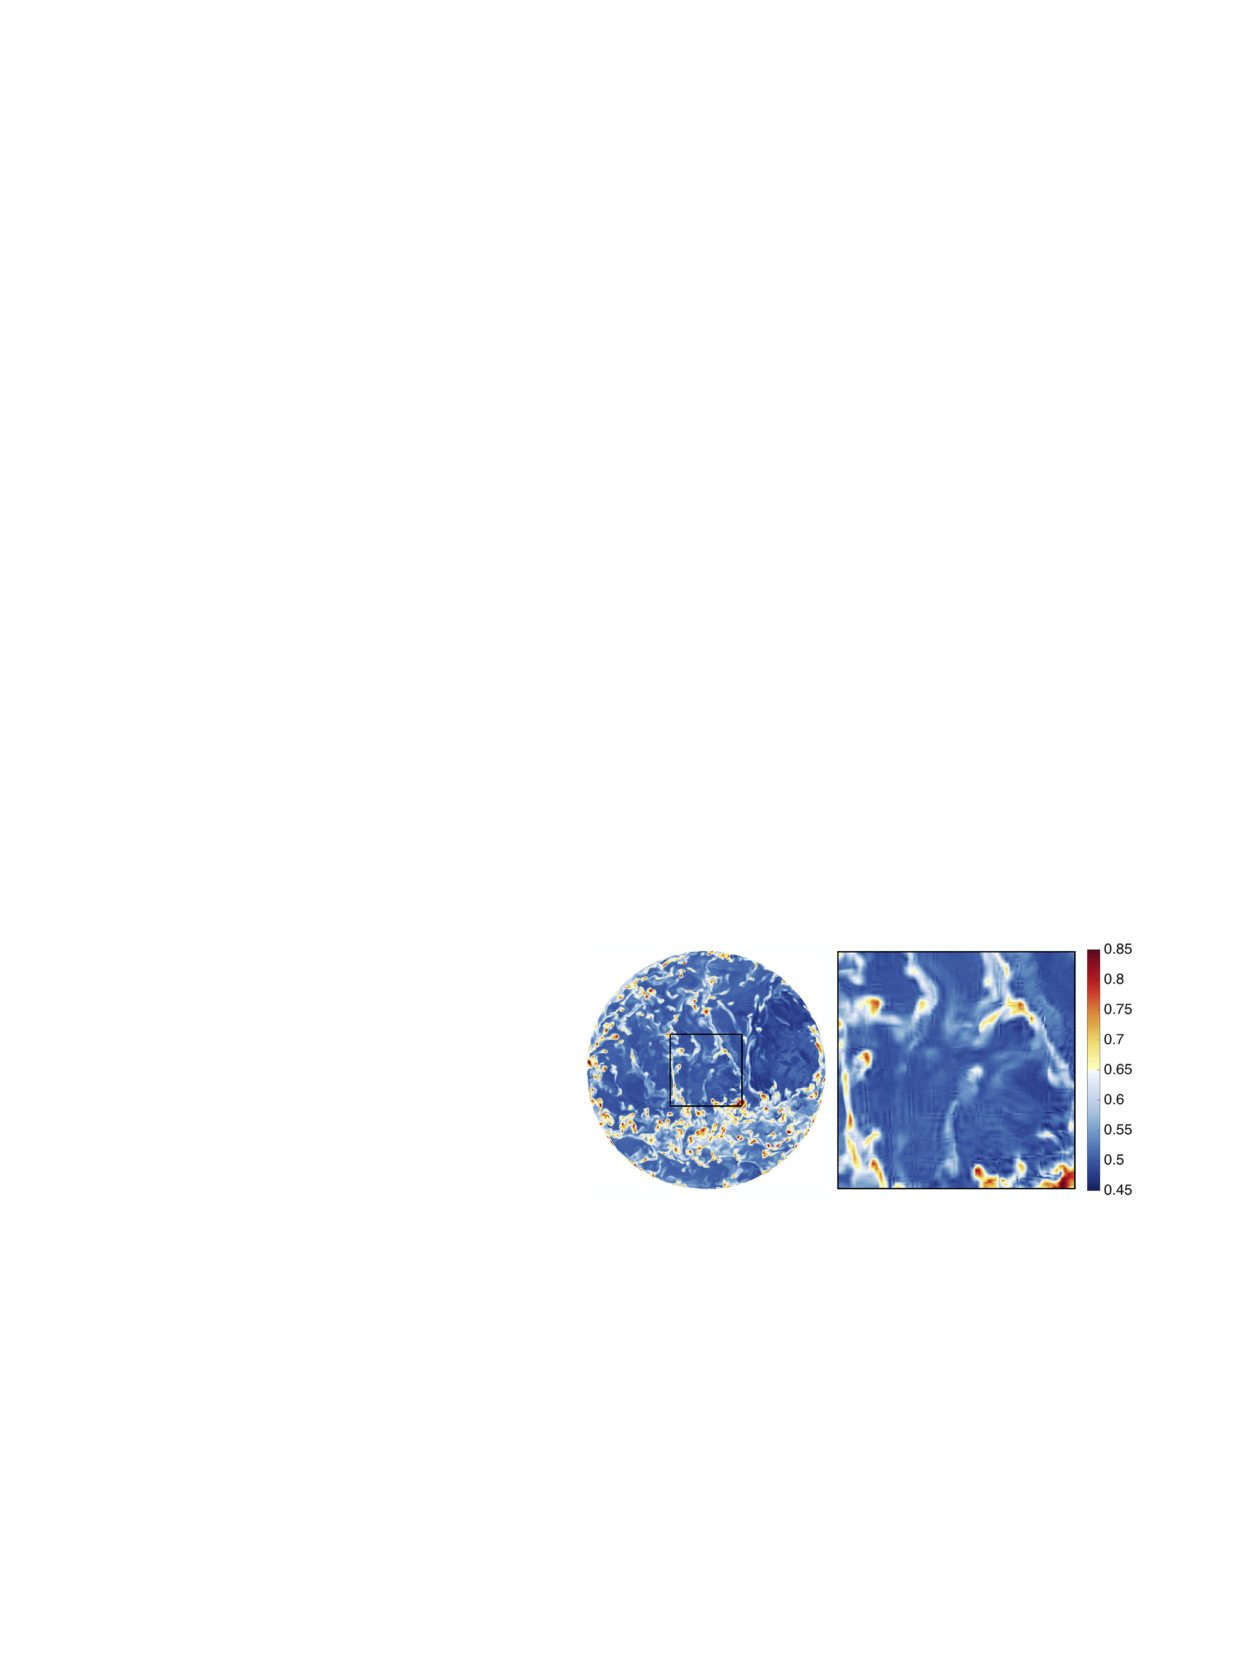
\includegraphics[width=\linewidth]{figures/kooij2018_artefacts.pdf}
    \caption{
        Reproduction of part of Figure 5 by \textcite{kooij2018}, showing an
        instantaneous horizontal temperature profile simulated by the
        \textsc{Nek}5000 code for \rb{} convection at $\rayleigh =
        \SI{e10}{}$. The profile is taken near the bottom plate of a
        cylindrical cavity and shows a grid-like pattern of numerical
        artefacts. The right panel is an enlargement of the region inside
        the black square in the left panel.
    }
    \label{fig:kooij2018_artefacts}
\end{figure}

\newpage
\section{Conclusion}

\newpage
\emergencystretch=5em
\printbibliography
\end{document}
